\section{Wednesday for MAT4002}\index{Monday_lecture}
\subsection{Remarks on Compactness}

\begin{theorem}
$X$ is compact, $Y$ is Hausdorff, $f:X\to Y$ is continuous and bijective. Then $X$ is \emph{homeomorphic} to $Y$
\end{theorem}

\begin{corollary}
If $X$ is compact, $Y$ is Hausdorff, $f:X\to Y$ is injective and continous, then
$f:X\to f(X)$ is homeomorphisc.
\end{corollary}
\begin{example}
Here we give another proof for the fact that $S^1\times S^1$ is homeomorphic to donut. Construct the mapping
\[
\begin{array}{ll}
f:&S^1\times S^1\to\mathbb{R}^3\\
\text{with}&(e^{i\theta},e^{i\phi})\mapsto((R+r\cos\theta)\cos\phi,(R+r\cos\theta)\sin\phi,r\sin\theta)\quad (R>r>0)
\end{array}
\]
Note that:
\begin{itemize}
\item
$X=S^1\times S^1$ is compact, $\mathbb{R}^3$ is Hausdorff;
\item
$f$ is continuous and injective.
\item
$f(S^1\times S^1)$ is a ``donut''.
\end{itemize}
Therefore, we conclude that $S^1\times S^1$ is homeomorphic to donut in $\mathbb{R}^3$.
\end{example}

\begin{definition}[Sequential Compactness]
A topological space $X$ is \emph{sequentially compact} if every sequence in $X$ has a convergent sub-sequence.
\end{definition}

In $\mathbb{R}^n$, the compactness is equivalent to sequential compactness. The same goes for any metric space $(X,d)$. (Check notes for MAT3006)

However, compactness and sequential compactness is different for topological spaces in general.

\subsection{Quotient Spaces}
\paragraph{Motivation}
Just like product space and disjoint union, we give another way to construct new topological spaces from some old ones. This new way of construction is by gluing some special pieces from old topological spaces together.
\paragraph{Idea}
Let $X=[0,1]\times[0,1]$ (just like a paper on a plane), we want to glue the leftmost edge with the rightmost edge to form a cylinder $Y_1$, as shown below:
\begin{figure}[H]
\centering
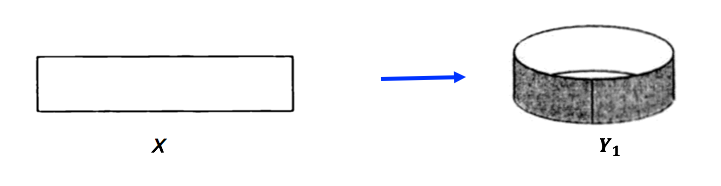
\includegraphics[width=0.7\textwidth]{week5/p_5}
\end{figure}
If we give a half-twist to the strip before glue the ends together, we will get the \emph{Moebius stripe} $Y_2$ shown below:
\begin{figure}[H]
\centering
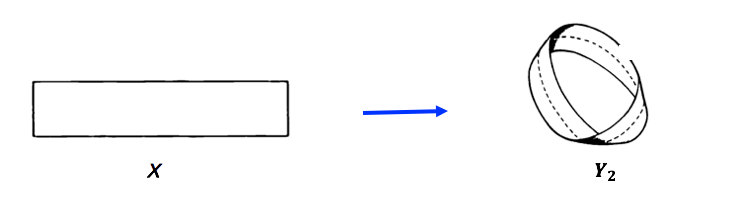
\includegraphics[width=0.7\textwidth]{week5/p_6}
\end{figure}
Interestingly, the first topology $Y_1$ has two sides, while the second has only one side.
\subsubsection{Equivalence Relations and partitions}
\begin{definition}[Equivalence Relation]
The \emph{equivalence} relation on a set $X$ is a relation $\sim$ such that 
\begin{enumerate}
\item
(Reflexive): $x\sim x,\forall x\in X$
\item
(Symmetric): $x\sim y$ implies $y\sim x$
\item
(Transitive): $x\sim y$ and $y\sim z$ implies $x\sim z$.
\end{enumerate}
\end{definition}

\begin{example}\label{exp:5:8}
\begin{enumerate}
\item
Let $X=V$ be a vector space, and $W\le V$ be a vector subspace. 
Define $\bm v_1\sim \bm v_2$ if $\bm v_1-\bm v_2\in W$.

(The well-definedness is left as exercise).
\item
(Mobius Stripe):
Let $X=[0,1]\times[0,1]$.
We define $(x_1,y_1)\sim(x_2,y_2)$ if 
\begin{itemize}
\item
$x_1=x_2, y_1=y_2$; (e.g., $(0.5,0.6)\sim(0.6,0.5)$) or
\item
$x_1=0,x_2=1,$ and $y_1=1-y_2$ (e.g., $(0,1/4)\sim(1,3/4)$)
\item
$x_1=1,x_2=0$, and $y_1=1-y_2$ (e.g., $(1,3/4)\sim(0,1/4)$)
\end{itemize}
\end{enumerate}
%\begin{enumerate}
%\item
%$P_i\subseteq X$ is non-empty
%\item
%$P_i\cap P_j=\emptyset$ if $i\ne j$
%\item
%$\bigcup_{i\in I}P_i=X$.
\end{example}
\begin{definition}[Partition]
Let $X$ be a nonempty set. A \emph{partition} $\mathcal{P}=\{p_i\mid i\in I\}$ of $X$ is a collection of subsets such that
\begin{enumerate}
\item
$P_i\subseteq X$ is non-empty
\item
$P_i\cap P_j=\emptyset$ if $i\ne j$
\item
$\bigcup_{i\in I}P_i=X$
\end{enumerate}
\end{definition}
\begin{remark}
Given a partition $\mathcal{P}$, we can define an equivalence relation $\sim$ on $X$ by setting
\[
x\sim y\quad
\text{whenever }x,y\in p_i,\text{ for some $i\in I$}
\]
For example, if $X=[0,1]\times[0,1]$, then 
\[
X=\{(x,y)\}_{x\in(0,1),y\in[0,1]}\cup\{(1,y),(0,1-y)\}_{y\in[0,1]}
\]
gives a partition on $X$. 
This gives the same equivalence relation as in part (2) in example~(\ref{exp:5:8}).
\end{remark}
Conversely, given an equivalence relation $\sim$, we could form a corresponding partition of $X$. This kind of partition is called the equivalence class:

\begin{definition}[Equivalence Class]
Let $X$ be a set with equivalence relation $\sim$. The equivalence class of an element $x\in X$ is
\[
[x]:=\{y\in X\mid x\sim y\}.
\]
\end{definition}
\begin{proposition}
The collection of all $[x]$ in $X/\sim$ gives a partition on $X$.
\end{proposition}
Consider the equivalence class defined in part (1) in example~(\ref{exp:5:8}). The equivalence class has the form
\[
[\bm v]= \{\bm u\in V\mid \bm v-\bm u\in W\}:=\bm v+W.
\]
Therefore, the equivalence class is a generalization of the \emph{coset} in linear algebra. Similarly, we define the set of generalized cosets as \emph{quotient space}.

\begin{definition}
The collection of all equivalence classes is called the \emph{quotient space}, denoted as $X/\sim$, i.e.,
\[
X/\sim = \{[x]\mid x\in X\}.
\]
\end{definition}

\begin{example}
\begin{enumerate}
\item
Consider part (1) in example~(\ref{exp:5:8}) again. The quotient space $V/\sim$ reduces to the $V/W$ in linear algebra:
\[
V/\sim = \{[\bm v]\mid \bm v\in V\}=\{\bm v+W\mid \bm v\in V\}=V/W.
\]
\item
Consider part (2) in example~(\ref{exp:5:8}) again. Then $X/\sim$ essentially forms the \emph{Mobius band}, e.g., 
\[
[(1/2,1/2)] = \{x\mid (1/2,1/2)\sim x\} = \{(1/2,1/2)\}
\]
\[
[(1,3/4)]=\{x\mid x\sim (1,3/4)\} = \{(1,3/4),(0,1/4)\}
\]
\end{enumerate}
\end{example}


\begin{example}
Consider $X=[0,1]\sqcup[0,1]$, i.e.,
\[
X = ([0,1]\times\{0\})\cup([0,1]\times\{1\})
\]
Take a partition on $X$ by 
\[
\{(a,0)\}_{0\le a<1}
\cup
\{(b,1)\}_{0<b\le1}
\cup
\{(1,0),(0,1)\}
\]
As a result, the corresponding quotient space is plotted below:
\begin{figure}[H]
\centering
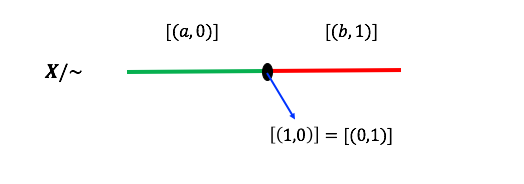
\includegraphics[width=0.7\textwidth]{week5/p_7}
\end{figure}
\end{example}


\begin{example}
Comes from $X=[0,1]\times[0,1]$ with partition 
\[
\{(a,b)\}_{0<a<1;0<b<1}\cup\{(x,0),(1-x,1)\}_{0\le x\le 1}
\cup\{(0,y),(1,1-y)\}_{0<y<1}
\]
The corresponding quotient space is plotted below:
\begin{figure}[H]
\centering
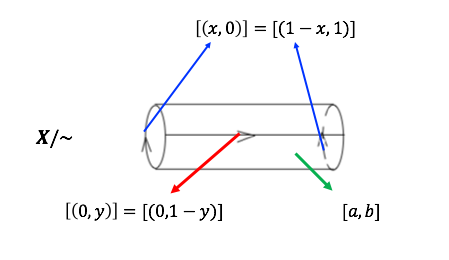
\includegraphics[width=0.5\textwidth]{week5/p_8}
\end{figure}
\end{example}

\begin{proposition}
Let $(X,\mathcal{T})$ be topological space, with the equivalence relation.
Define the canonical projection map
\[
\begin{array}{ll}
p:&X\to X/\sim\\
\text{with}&x\mapsto[x]
\end{array}
\]
Define a collection of subsets $\tilde{\mathcal{T}}$ on $X/\sim$ by:
\[
\text{$U\subseteq X/\sim$ is in $\tilde{\mathcal{T}}$ if $p^{-1}(U)$ is in $\mathcal{T}.$}
\]
Then $\tilde{\mathcal{T}}$ is a topology for $X/\sim$, called \emph{quotient topology}.
\end{proposition}



























